Besides Bravais classes, neural networks and graph neural networks, the fourth ingredient for this report is a percolation.
We start with an undirected graph $G=(V,E)$ and want to define what paths and cycles are. Pick two nodes $n_1, n_2\in V$. We say that $n_1$ and $n_2$ are connected if
there are nodes $m_0,m_1,\dots,m_N\in V$ such that $m_0=n_1$, $m_N=n_2$ and for each $i\in\{0,\dots,N-1\}$ there is an edge $\{m_i,m_{i+1}\}\in E$.
In this case, the tuple $(m_0,m_1,...,m_N)$ is called a path of length $N$ from $n_1$ to $n_2$. A path is $(m_0,m_1,...,m_N)$ is called a cycle if $m_i\neq m_j$ for $i\neq j$ (i.e. no node is visited twice).

Knowing what paths and cycles are, everything is set up to introduce percolating graph. Suppose $G=(V,E)$ is an undirected graph, 
where each node $n\in V$ has a position $p_n=(n_x,n_y)\in[0,1]\times[0,1]$. Visually, we think of $G$ as a graph inside the unit square.
Fix $\frac{1}{2}>r>0$. The graph is called percolating, if there are nodes $n,m\in V$ such that
\begin{enumerate}
    \item there is a cycle containing $n$ and $m$,
    \item $\{n,m\}\in E$ and
    \item either $n_x<r$ and $m_x>1-r$ or $n_y<r$ and $m_y>1-r$.
\end{enumerate}
Figure~\ref{fig:percolation_example} gives an example of percolating and non-percolating graphs. 
Properties 1. and 2. are easily understood. It is worth mentioning, that 1. and 2. imply, that there is a cycle containing $n$,$m$ as well as the edge $\{n,m\}$.
Property 3. needs a bit more explanation: We can picture small trips of width $r$ at the sides of the unit square 
(see figure~\ref{fig:percolation_example} where the strips are colored red and blue), Requiring $n_x<r$ and $m_x>1-r$ means that $n$ is located on the left side of the unit square while
$m$ is located on the right side. 
Accordingly, $n_y<r$ and $m_y>1-r$ requires $n$ to be on the bottom and $m$ to be on the top of the unit square.
In any of these two cases, $n$ and $m$ are in strips of the same color but on opposite sites.
The restriction to $r<\frac{1}{2}$ guarantees that strips of the same color do not overlap.
\begin{figure}
    \centering
    %\hfill
    \begin{subfigure}[t]{0.44\textwidth}
        \centering
        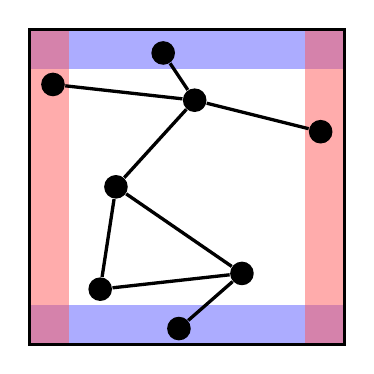
\begin{tikzpicture}[
            node/.style={circle, inner sep=0pt, fill=black, minimum size=3mm}
        ]
        \fill[blue!65, fill opacity=0.5] (0,0) rectangle (4, 0.5);
        \fill[blue!65, fill opacity=0.5] (0,3.5) rectangle (4, 4);
        \fill[red!65, fill opacity=0.5] (0,0) rectangle (0.5, 4);
        \fill[red!65, fill opacity=0.5] (3.5,0) rectangle (4, 4);
        \draw[black, very thick] (0,0) rectangle (4,4);
        \node[node] at (0.3, 3.3) (n1) {};
        \node[node] at (1.1, 2.0) (n2) {};
        \node[node] at (0.9, 0.7) (n3) {};
        \node[node] at (2.7, 0.9) (n4) {};
        \node[node] at (2.1, 3.1) (n5) {};
        \node[node] at (3.7, 2.7) (n6) {};
        \node[node] at (1.7, 3.7) (n7) {};
        \node[node] at (1.9, 0.2) (n8) {};
        \draw[very thick]  (n1) -- (n5);
        \draw[very thick]  (n5) -- (n2);
        \draw[very thick]  (n5) -- (n6);
        \draw[very thick]  (n2) -- (n4);
        \draw[very thick]  (n3) -- (n4);
        \draw[very thick]  (n2) -- (n3);
        \draw[very thick]  (n5) -- (n7);
        \draw[very thick]  (n8) -- (n4);
        \end{tikzpicture}
        \caption{non-percolating graph}
    \end{subfigure}
    %\hfill
    \begin{subfigure}[t]{0.55\textwidth}
        \centering
        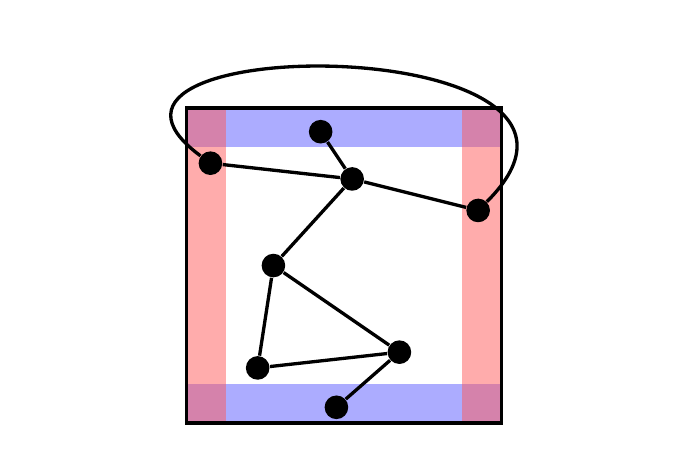
\begin{tikzpicture}[
            node/.style={circle, inner sep=0pt, fill=black, minimum size=3mm}
        ]
        \fill[blue!65, fill opacity=0.5] (0,0) rectangle (4, 0.5);
        \fill[blue!65, fill opacity=0.5] (0,3.5) rectangle (4, 4);
        \fill[red!65, fill opacity=0.5] (0,0) rectangle (0.5, 4);
        \fill[red!65, fill opacity=0.5] (3.5,0) rectangle (4, 4);
        \draw[black, very thick] (0,0) rectangle (4,4);
        \node[node] at (0.3, 3.3) (n1) {};
        \node[node] at (1.1, 2.0) (n2) {};
        \node[node] at (0.9, 0.7) (n3) {};
        \node[node] at (2.7, 0.9) (n4) {};
        \node[node] at (2.1, 3.1) (n5) {};
        \node[node] at (3.7, 2.7) (n6) {};
        \node[node] at (1.7, 3.7) (n7) {};
        \node[node] at (1.9, 0.2) (n8) {};
        \draw[very thick]  (n1) -- (n5);
        \draw[very thick]  (n5) -- (n2);
        \draw[very thick]  (n5) -- (n6);
        \draw[very thick]  (n2) -- (n4);
        \draw[very thick]  (n3) -- (n4);
        \draw[very thick]  (n2) -- (n3);
        \draw[very thick]  (n5) -- (n7);
        \draw[very thick]  (n8) -- (n4);
        \draw[very thick]  (n1) .. controls (-2,5) and (6,5) .. (n6);
        \end{tikzpicture}
        \caption{percolating graph}
    \end{subfigure}
    
    \caption{Illustration of percolating and non-percolating graphs.}
    \label{fig:percolation_example}
\end{figure}